\documentclass{beamer}

\usetheme[]{Rochester}
\usecolortheme{beaver}
\usepackage[latin1]{inputenc}
\usepackage{graphics}

\author{Will Webberley}
\date{Autumn 2014}
\institute[COMSC]{Cardiff School of Computer Science and Informatics}



\title{User-Centric Interaction Engineering}
\subtitle{CM2101: Human-Computer Interaction}

\begin{document}

\frame{\titlepage}

\frame{
    \frametitle{What is an interface?}
    Generally, it is the plane of interaction between two media.
    \begin{description}[1980-2000]
        \item[1950-60] Interface at hardware only
        \item[1960-70] Interface at programming level
        \item[1970-80] Interface at terminal level
        \item[1980-2000] Interface at interaction dialogue (graphical displays)
        \item[2000-10] Interface becomes pervasive (RF tags, consumer electronics, embedded devices)
        \item[2010+] Interface replaced by \alert{experiences} (focus on tasks, emotions, elegance, social connections)
    \end{description}
}

\frame{
    \frametitle{}
    \centering{
        Therefore, we consider \alert{interaction design} instead of simply \alert{interface design}
    }
}

\frame{
    \frametitle{Users}
    The problem with users:
    \begin{itemize} 
        \item Systems typically have them 
        \item They're always `right'
        \item Users aren't the enemy
        \item Users aren't all the same
        \item Users can be prompted and instructed     
    \end{itemize}
}

\frame{
    \frametitle{User interaction}   
    Many interactions are small, but important:
    \begin{itemize}
        \item Automatic door
        \item Lift
        \item Travel ticket barrier
        \item Central heating
        \item Fridge
        \item Coffee machine
    \end{itemize}
    Designers need to consider the feedback loop to users.    
}

\frame{
    \frametitle{HCI design constraints}
    \centering
    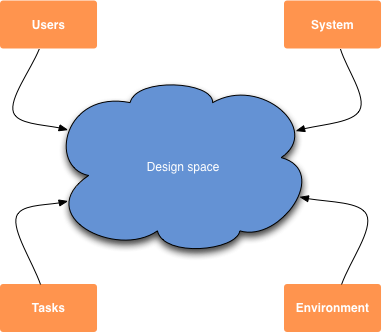
\includegraphics[height=7cm]{media/constraints.png}   
}

\frame{
    \frametitle{Software development cycle}
    \begin{itemize}
        \item HCI is a key part of the software development cycle
        \item HCI also needs its own development cycle
        \item HCI aspects are drawn from the \alert{functional requirements} of a system
        \item If there is a task the user needs to do, then the system must allow it
        \item Tasks can be \alert{dynamically prioritised} through menus and options
    \end{itemize}
}

\frame{
    \frametitle{Waterfall: Traditional development cycle}
    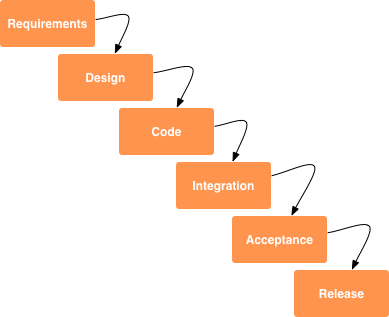
\includegraphics[height=7cm]{media/waterfall.png}   
}

\frame{
    \frametitle{Waterfall: Traditional development cycle}  
    \begin{itemize}
        \item Each `iteration' becomes a release
        \item Effectively end-users become testers
        \item By this stage, it's too late
        \item If users don't like it, then they won't come back for future versions
    \end{itemize}
}

\frame{
    \frametitle{Waterfall: Traditional development cycle}
    Therefore, the waterfall is inappropriate for usability engineering, since:
    \begin{itemize}
        \item Design is likely to be `wrong' the first few times
        \item No user testing until the end
        \item Wasted effort on code written that needs to be thrown out
    \end{itemize}
    \vskip20pt
    Usability engineering needs to be much more agile:
    \begin{itemize}
        \item Iterative
        \item User-centric from the beginning
    \end{itemize}
}

\frame{
    \frametitle{Iterative and user-centric design}
    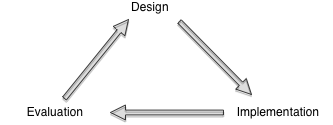
\includegraphics[height=4cm]{media/cycle.png}   
}

\frame{
    \frametitle{Iterative design}
    \begin{itemize}
        \item Use \alert{cheap} prototypes (whiteboards, paper, etc.) for \alert{early} iterations
        \item Use \alert{richer} prototypes later when \alert{changes become smaller}
        \item Ensure the `world' only sees mature iterations
        \item The more iterations: higher quality UX
    \end{itemize}   
}

\frame{
    \frametitle{User-centric design}
    \begin{itemize}
        \item Focus on the anticipated \alert{audience}
        \item Keep in mind the \alert{goals} and \alert{tasks} the users will need to do
        \item \alert{Consult} users in \alert{each} iteration
        \item Involve non-developmental users as \alert{evaluators} in \alert{each} iteration
        \item Keep in mind \alert{human factors} and the abilities of the users
    \end{itemize}
}

\frame{
    \frametitle{LUCID framework}
    \alert{Logical User-Centred Interaction Design}
    \textit{- Charlie Kreizberg, Cognetics Corporation}
    \vskip20pt
    A framework for \alert{guiding} and managing the process of user interaction design
}

\frame{
    \frametitle{LUCID framework}
    \alert{Logical}
    \begin{itemize}
        \item Design process built on strong \alert{conceptual model}
        \item Iterative review and refinement
        \item Successive prototyping and team reviews
    \end{itemize}
    \alert{User-Centred}
    \begin{itemize}
        \item Designed from the system tasks and workflow
        \item Design based on user activity and context
        \item Users provide feedback throughout
    \end{itemize}
    \alert{Interaction Design}
    \begin{itemize}
        \item Distinct from technical design
        \item `Everything but code' approach
    \end{itemize}
}

\frame{
    \frametitle{LUCID framework: 6 stages}
    \begin{enumerate}
        \item Envision
        \begin{itemize}
            \item Develop \alert{UI roadmap} that defines the concept, constraints, and design objectives
        \end{itemize}
        \item Analyse
        \begin{itemize}
            \item Analyse user needs and develop \alert{requirements}
        \end{itemize}
        \item Design
        \begin{itemize}
            \item Create a low-fidelity \alert{design concept}
        \end{itemize}
        \item Refine
        \begin{itemize}
            \item \alert{User-test} and \alert{evaluate} the prototype for design problems and refine design
        \end{itemize}
        \item Implement
        \begin{itemize}
            \item \alert{Support implementation} of system, making last-minute small changes if required
        \end{itemize}
        \item Support
        \begin{itemize}
            \item Provide rollout support as product is deployed
            \item \alert{Collect data} for new version
        \end{itemize}
    \end{enumerate}
}

\frame{
    \frametitle{LUCID framework: 6 stages}
    \centering{
        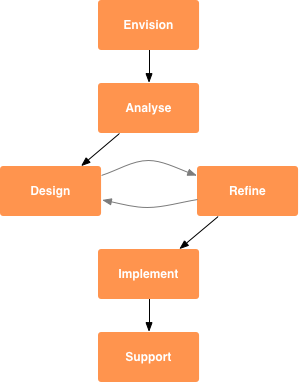
\includegraphics[height=7cm]{media/lucid.png}
    } 
}

\frame{
    \frametitle{User evaluation}
    \alert{User evaluation} is the first interaction evaluation studied on this course.
    This will be useful for your first coursework, but there are also other techniques we'll cover later.
    \vskip10pt
    \centering{
        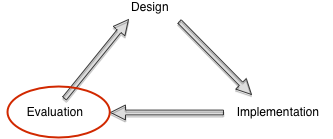
\includegraphics[height=4cm]{media/cycle_2.png}
    }
}

\frame{
    \frametitle{User evaluation: `think aloud'}
    Generally: a user speaks their thoughts whilst completing a task.
    \begin{block}{Think aloud recipe}
        \begin{enumerate}
            \item Tester selects a task to be completed for a given system
            \item Tester is told what they are required to do
            \item User is given access to the system's interface
            \item User navigates through the system and tries to complete the task
            \item User speaks \alert{all} thoughts aloud
            \item Tester records all spoken thoughts for later evaluation 
        \end{enumerate}
    \end{block}
}

\frame{
    \frametitle{User evaluation: `think aloud'}
    \begin{itemize}
        \item User should try and speak aloud all thoughts
        \begin{itemize}
            \item Frustrations (``Ugh... Why did \textit{that} happen?'')
            \item What they think is happening
            \item What they're trying to do
            \item Messages encountered (and perception of these)
            \item Why a particular action was taken (``I tapped here because...'')
            \item Things that are confusing (``What's the difference between these two options?'')
            \item Questions that arise in the mind
        \end{itemize}
        \item Tester should stay quiet and shouldn't respond to questions
        \item If user is quiet, tester should prompt (``Why did you tap that?'', ``What are you thinking?'')
    \end{itemize}
}

\frame{
    \frametitle{`Think aloud' method}
    \begin{columns}
        \column{.5\textwidth}
            \begin{block}{Pros}
                \begin{itemize}
                    \item Gives insights into thoughts
                    \item Usable in early iterations
                    \item Understand what the interface \textit{says} to the user
                    \item Understand what feels natural to the user and what doesn't
                    \item Highlights areas of frustration or confusion
                    \item Widely-used evaluation method
                \end{itemize}
            \end{block}
        \column{.5\textwidth}
            \begin{block}{Cons}
                \begin{itemize}
                    \item May alter the way users approach the task
                    \item It feels unnatural
                    \item Hard to talk if concentrating
                    \item Tasks take longer (slows by about 17\%)
                \end{itemize}
            \end{block}
    \end{columns}
}

\frame{
    \frametitle{`Think aloud' setup}
    \begin{itemize}
        \item User should have the procedure and test explained to them
        \item User should be relaxed
            \begin{itemize}
                \item Demo `think aloud' using unrelated task (e.g. looking up train times)
                \item User should practice using an unrelated task
            \end{itemize}
        \item Ensure quiet, comforable room. Turn phones to silent and prevent anticiapted interruptions.
        \item Test may be recorded visually 
    \end{itemize}
}

\frame{
    \frametitle{After a `think aloud' test}
    \begin{itemize}
        \item Use notes to evaluate performance of interactions
        \item Where were there positive thoughts? (``This makes sense'', ``That's what I thought would happen'')
        \item Where were there negative thoughts? (``How am I supposed to be able to do this?'')
        \item Use notes to help improve next iteration
    \end{itemize}
}

\frame{
    \frametitle{`Think aloud' demo}
}

\frame{
    \frametitle{Revision questions}
    \begin{enumerate}
        \item In what systems is HCI important?
        \item What is \textit{usability} in the context of HCI?
        \item Describe 3 important aspects of HCI that are important to consider when designing interactions.
        \item Why is human \textit{diversity} important to consider when designing interactions?
        \item What are key differences between user \textit{interfaces} and user \textit{interactions}?
        \item Why is the waterfall model unsuitable for interaction design?
        \item What are the main benefits of using \textit{iterative} design?
        \item Why are \textit{users} very important in interaction design?
        \item Provide a general overview of the LUCID framework for interaction design.
        \item Describe the process of the `think aloud' user evaluation test. In what ways is it useful? 
    \end{enumerate}
}

\frame{
    \frametitle{Summary}
    \begin{itemize}
        \item Differences between user \alert{interfaces} and \alert{interactions}
        \item Consideration of users in all systems
        \item The inappropriateness of the traditional software development cycle for usability engineering
        \item The importance of \alert{iterative} and \alert{user-centric} design
        \item The LUCID framework
        \item `Think aloud' user evaluation
    \end{itemize}
}

\end{document}
